% !TEX TS-program = xelatex
% !TEX encoding = UTF-8 Unicode
% !Mode:: "TeX:UTF-8"

\documentclass{resume}
\usepackage{zh_CN-Adobefonts_external} % Simplified Chinese Support using external fonts (./fonts/zh_CN-Adobe/)
% \usepackage{NotoSansSC_external}
% \usepackage{NotoSerifCJKsc_external}
% \usepackage{zh_CN-Adobefonts_internal} % Simplified Chinese Support using system fonts
\usepackage{linespacing_fix} % disable extra space before next section
\usepackage{cite}
\usepackage{graphicx}%插入图片
\usepackage{tabularx,booktabs}%控制版面
\usepackage{float}%控制图片位置
\usepackage{setspace}% 调整行间距
\usepackage{multicol}%分栏
\usepackage{geometry}%设置页边距
\usepackage{fontawesome}%特殊符号,以\fa开头
\usepackage{multirow}%合并行
\usepackage{makecell}%合并行
\usepackage{array}%设置表格行距

\geometry{left=1.0cm,right=1.0cm,top=1.0cm,bottom=1.0cm}

\begin{document}
  \begin{minipage}[b]{0.8\linewidth}
    {\Huge \heiti 蒋贤伟}\\
    \ \textperiodcentered\ 
    \email{\  vanot313@gmail.com}\\
    \ \textperiodcentered\ 
    \phone{\  199-6730-0606}\\
    \ \textperiodcentered\ 
    \github[\  vanot313]{https://github.com/vanot313}
  \end{minipage}
  \hfill
  \begin{minipage}[t]{0.2\linewidth}
  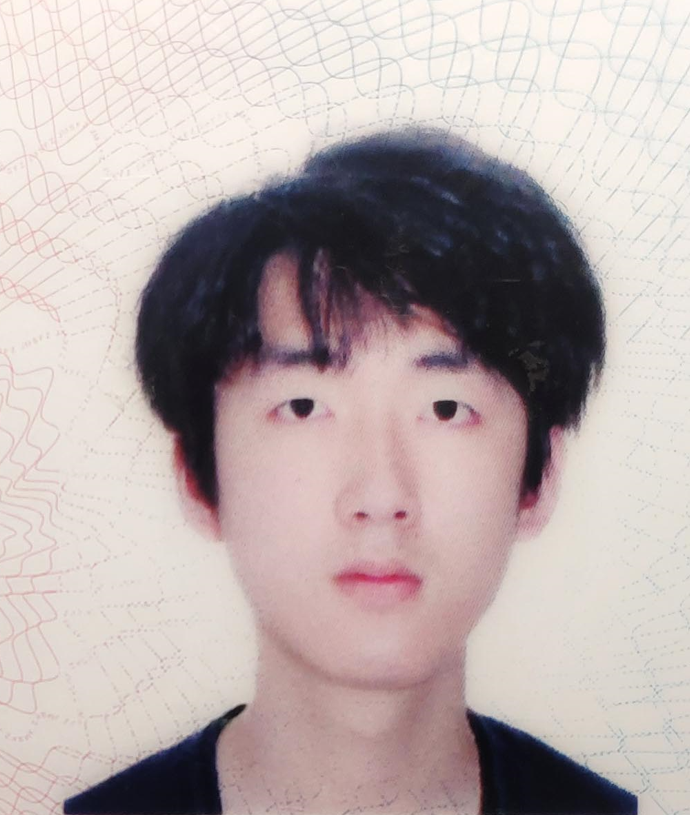
\includegraphics[height=5\baselineskip]{head.png}
  \end{minipage}

  \section{\faGraduationCap\ 教育背景}
  \datedsubsection{\textbf{浙江工业大学}, 杭州}{2018 年 9 月 -- 至今}
  \datedsubsection{\textit{在读本科学士}\ 软件工程, 预计 2022 年 6 月毕业}{GPA 3.5(TOP 30\%)}

  \section{\faUsers\ 项目经历}

  \datedsubsection{\textbf{第十二届中国大学生服务外包创新创业大赛}}{2021 年 1 月 -- 2021 年 5 月}
  \role{https://github.com/vanot313/project-data\_asset\_valuation-BC}{团队项目,担任队长}
  \begin{onehalfspacing}
  Flask 后端应用
    \begin{itemize}
      \item 完成 flask 应用的 MVC 框架设计与权限验证安全实现。在框架的支撑下后台应用表现出优良的可拓展性,
      注册路由后编写功能接口或是数据接口可以完成大部分业务的拓展。
      \item 采用 mysql 作为数据库,根据业务需求完成数据表,视图设计。设计基本触发器逻辑。
    \end{itemize}
  完整项目在服务端(ubuntu)的部署上线
    \begin{itemize}
      \item 采用 docker 自动化配置服务端环境,docker-compose 配置完成前后端应用的联合部署。
      \item 采用 nginx 反向代理服务器,监听80端口,uWSGI 服务器部署后台应用集群分布在其他端口,
      完成应用在服务端的集群部署。
    \end{itemize}
  
  \end{onehalfspacing}

  \datedsubsection{\textbf{网易 MiniGame 游戏大赛}}{2020 年 9 月 -- 2020 年 11 月}
  \role{https://github.com/SharpLeaves/Core}{团队项目,担任程序兼策划}
  \begin{onehalfspacing}
  Unity 横板过关游戏
    \begin{itemize}
      \item 负责游戏创意策划,完成游戏中关卡创意部分的实现(场景角色的行为逻辑,与场景的交互逻辑)
      \item 完成游戏框架(状态机,人物碰撞模型与碰撞逻辑)编写,编写了框架的介绍文档并上传在 github 仓库。
    \end{itemize}
  \end{onehalfspacing}

  \datedsubsection{\textbf{健康码管理系统}}{2020 年 5 月 -- 2020 年 7 月}
  \role{https://github.com/vanot313/design-xhealthcode-BC}{个人项目}
  \begin{onehalfspacing}
  JavaWeb 全栈开发
  \begin{itemize}
    \item 完成底层 IoC/DI 容器(仿照 Spring)以及完整后台系统框架与功能的编写,利用 java 反射的机制,
    完成通过接口对容器注入服务的功能。    
  \end{itemize}
  \end{onehalfspacing}


  \section{\faCogs\ IT 技能}
  \begin{itemize}[parsep=0.5ex]
    \item 熟悉 Java、Python,了解 C++,熟悉数据结构与基本算法(阅读过 java Collection 集合源代码)
    \item 熟悉 Flask 框架、SSM、Springboot框架,了解 Vue 前端生态
    \item 熟悉 Docker,Nginx 等项目部署相关知识,了解 Linux 环境下操作
    % \item 了解深度学习基本算法,LSTM长短时记忆神经网络
  \end{itemize}

  \section{\faHeartO\ 获奖情况}
  \begin{itemize}[parsep=0.5ex]
    \item \datedline{\textit{银奖}, ACM程序设计校迎新赛}{2018 年 11 月}
    \item \datedline{\textit{三等}, 校奖学金}{2018 年 - 2020 年}
    \item \datedline{\textit{二作}, 软件著作权}{2021 年}
  \end{itemize}

  \section{\faInfo\ 其他}
  \begin{itemize}[parsep=0.5ex]
    \item 参与学院学生会工作两年(负责学院创新分服务器以及微信公众号的开发与维护)
    \item 个人博客网站: http://vanot313.top (建设中,采用 Springboot 框架)
    \item 语言: 英语 - 熟练(CET 6)
    % \item 热爱技术,喜欢用技术的方式来解决问题,例如这篇简历就是用 LaTex 完成的。
  \end{itemize}
  
\end{document}
